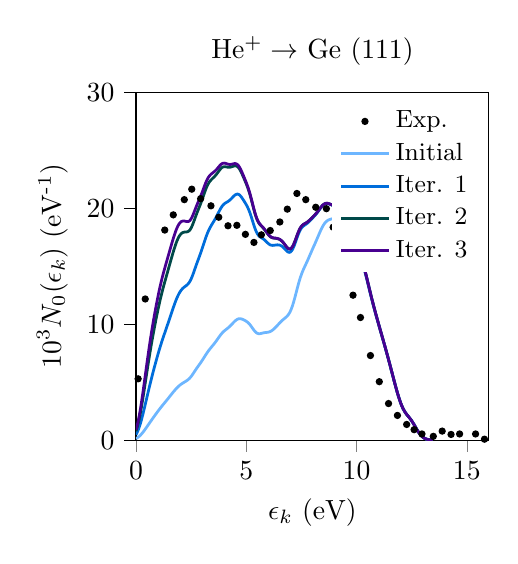
\begin{tikzpicture}

\begin{axis}[
width=0.5\textwidth,
height=6cm,
legend cell align={left},
tick align=outside,
tick pos=left,
title={He$^+ \rightarrow$ Ge (111)},
xlabel={\(\displaystyle \epsilon_k\) (eV)},
xmin=0, xmax=16,
ylabel={\(\displaystyle 10^3 N_0\)($\epsilon_k$) (eV\textsuperscript{-1})},
ymin=0, ymax=30,
ytick style={color=black},
legend style={%
draw=white!80.0!black, draw=none, font=\small
},
]
% This file was created by tikzplotlib v0.9.1.
\definecolor{color0}{rgb}{0.427450980392157,0.713725490196078,1}
\definecolor{color1}{rgb}{0,0.427450980392157,0.858823529411765}
\definecolor{color2}{rgb}{0.282352941176471,0,0.568627450980392}

\addplot [semithick, black, mark=*, mark size=1, mark options={solid}, only marks]
table {%
0.0966442953020134 5.28688524590164
0.418791946308725 12.172131147541
1.30469798657718 18.1147540983607
1.69127516778523 19.4262295081967
2.19060402684564 20.7377049180328
2.52885906040268 21.6393442622951
2.93154362416107 20.8196721311475
3.39865771812081 20.2049180327869
3.75302013422819 19.2213114754098
4.17181208053691 18.4836065573771
4.5744966442953 18.5245901639344
4.96107382550336 17.7459016393443
5.34765100671141 17.0491803278689
5.68590604026845 17.7049180327869
6.08859060402685 18.0737704918033
6.52348993288591 18.8114754098361
6.86174496644295 19.9180327868852
7.29664429530201 21.2704918032787
7.6993288590604 20.7377049180328
8.1503355704698 20.0819672131148
8.63355704697987 19.9590163934426
8.93959731543624 18.3606557377049
9.39060402684564 15.983606557377
9.84161073825503 12.5
10.1798657718121 10.5737704918033
10.6308724832215 7.29508196721311
11.0335570469799 5.04098360655738
11.4523489932886 3.15573770491803
11.855033557047 2.13114754098361
12.2738255033557 1.35245901639344
12.6120805369128 0.901639344262295
12.9664429530201 0.532786885245898
13.4818791946309 0.327868852459015
13.8845637583893 0.778688524590164
14.2872483221477 0.491803278688525
14.6738255033557 0.532786885245898
15.3986577181208 0.532786885245898
15.8013422818792 0.0819672131147522
};
\addlegendentry{Exp.}
\addplot [line width=1pt, color0]
table {%
-0.00119532954451529 0.133856117758139
0.0488046704554819 0.187181127091969
0.0988046704554826 0.253151999571489
0.148804670455483 0.332008969556958
0.198804670455484 0.42338802476586
0.248804670455485 0.526383166630717
0.298804670455482 0.639653378421604
0.348804670455483 0.761545088473834
0.398804670455483 0.890215872181102
0.448804670455484 1.0237614224787
0.498804670455485 1.16035114448787
0.548804670455482 1.29836829043009
0.598804670455483 1.43653270614953
0.648804670455483 1.57397256182631
0.698804670455484 1.71022109370701
0.748804670455485 1.84513672313498
0.798804670455482 1.9787697435503
0.848804670455483 2.11121168238885
0.898804670455483 2.24246285882069
0.948804670455484 2.37234839658781
0.998804670455485 2.50050573456063
1.04880467045548 2.62646096091497
1.09880467045548 2.74979095897616
1.14880467045548 2.87032876460107
1.19880467045548 2.98832934754668
1.24880467045548 3.10450355166943
1.29880467045548 3.21987313041916
1.34880467045548 3.33548747856004
1.39880467045548 3.45212076178065
1.44880467045548 3.57008277853711
1.49880467045548 3.68921196435482
1.54880467045548 3.80900605963248
1.59880467045548 3.92877395718352
1.64880467045548 4.04769654565648
1.69880467045548 4.16477730111249
1.74880467045548 4.27876055287918
1.79880467045548 4.38814527519055
1.84880467045548 4.49136751740071
1.89880467045548 4.58711362874346
1.94880467045548 4.67462978577959
1.99880467045548 4.75388340653664
2.04880467045548 4.82552334278163
2.09880467045548 4.89071906028598
2.14880467045548 4.95104598569015
2.19880467045548 5.00854586176773
2.24880467045548 5.06594074518087
2.29880467045548 5.12680381219672
2.34880467045548 5.19541569973562
2.39880467045548 5.2761299949199
2.44880467045548 5.3723248906253
2.49880467045548 5.48529397625361
2.54880467045548 5.61356559849584
2.59880467045548 5.75304624756845
2.64880467045548 5.89807048311406
2.69880467045548 6.04304890735744
2.74880467045548 6.18412025942612
2.79880467045548 6.32017904414924
2.84880467045548 6.45288580325877
2.89880467045548 6.58566815123713
2.94880467045548 6.72212443926242
2.99880467045548 6.86446689644775
3.04880467045548 7.01259468093115
3.09880467045548 7.16410894531052
3.14880467045548 7.31517931039591
3.19880467045548 7.46184924019427
3.24880467045548 7.60124466917077
3.29880467045548 7.73227029965047
3.34880467045548 7.85566218257697
3.39880467045548 7.97354569787688
3.44880467045548 8.08878681716665
3.49880467045548 8.20438717556891
3.54880467045548 8.32300048719982
3.59880467045548 8.44650617238582
3.64880467045548 8.57556918067599
3.69880467045548 8.70923587754645
3.74880467045548 8.84477420927638
3.79880467045548 8.97799333788309
3.84880467045548 9.10413259408697
3.89880467045548 9.21912800997285
3.94880467045548 9.320836152065
3.99880467045548 9.40974783774539
4.04880467045548 9.48890690723974
4.09880467045548 9.56306909070792
4.14880467045548 9.63742050312247
4.19880467045548 9.71630178230643
4.24880467045548 9.8022972859046
4.29880467045548 9.89583517977669
4.34880467045548 9.99522898501125
4.39880467045548 10.0969886872174
4.44880467045548 10.1962631835832
4.49880467045548 10.2873862515984
4.54880467045548 10.3645870231902
4.59880467045548 10.4228892144677
4.64880467045548 10.4590819944872
4.69880467045548 10.4724704598656
4.74880467045548 10.4650572294642
4.79880467045548 10.4409258679887
4.84880467045548 10.4048982474408
4.89880467045548 10.3608790091754
4.94880467045548 10.3104941602977
4.99880467045548 10.2525867398316
5.04880467045548 10.1838221518287
5.09880467045548 10.1002305485029
5.14880467045548 9.99916311184714
5.19880467045548 9.88098258184421
5.24880467045548 9.74992186202209
5.29880467045548 9.61383054410665
5.34880467045548 9.48287232275404
5.39880467045548 9.36752684457271
5.44880467045548 9.27642825010386
5.49880467045548 9.21459311811291
5.54880467045548 9.18250092713572
5.59880467045548 9.17624802456582
5.64880467045548 9.18870750322087
5.69880467045548 9.21135800892618
5.74880467045548 9.23628500759098
5.79880467045548 9.25786071178089
5.84880467045548 9.27373891399044
5.89880467045548 9.28500251351663
5.94880467045548 9.29549392260355
5.99880467045548 9.31054073433563
6.04880467045548 9.33542026242097
6.09880467045548 9.37399335560631
6.14880467045548 9.42789186758798
6.19880467045548 9.49646797112959
6.24880467045548 9.57742439598166
6.29880467045548 9.66776997964896
6.34880467045548 9.7646437465834
6.39880467045548 9.86565596415238
6.44880467045548 9.96872332196986
6.49880467045548 10.0716546717192
6.54880467045548 10.1719151459665
6.59880467045548 10.2669057906197
6.64880467045548 10.3547983806597
6.69880467045548 10.435663899826
6.74880467045548 10.5124156531384
6.79880467045548 10.5911311423408
6.84880467045548 10.6805411462249
6.89880467045548 10.7907845082635
6.94880467045548 10.9317709608755
6.99880467045548 11.1115483334306
7.04880467045548 11.3349793832825
7.09880467045548 11.6028629818208
7.14880467045548 11.911520131014
7.19880467045548 12.2528840815177
7.24880467045548 12.6151642567337
7.29880467045548 12.9841716895562
7.34880467045548 13.3452606240582
7.39880467045548 13.6856164864779
7.44880467045548 13.9963969022341
7.49880467045548 14.2741571796
7.54880467045548 14.5211113442943
7.59880467045548 14.7440989868749
7.64880467045548 14.9525183452324
7.69880467045548 15.1558051141527
7.74880467045548 15.3611875863027
7.79880467045548 15.5723473011761
7.84880467045548 15.7893178081462
7.89880467045548 16.0095348334144
7.94880467045548 16.229585538416
7.99880467045548 16.4469796887975
8.04880467045548 16.6612782406679
8.09880467045548 16.8741665675165
8.14880467045548 17.0884646694273
8.19880467045548 17.3065051341861
8.24880467045548 17.5285652177882
8.29880467045548 17.7520291085919
8.34880467045548 17.9716056457108
8.39880467045548 18.1804741790164
8.44880467045548 18.371818363421
8.49880467045548 18.5401728811165
8.54880467045548 18.6822082249762
8.59880467045548 18.7969402624074
8.64880467045548 18.8855985285008
8.69880467045548 18.9513626031958
8.74880467045548 18.9990095175079
8.79880467045548 19.0343734146563
8.84880467045548 19.063519912035
8.89880467045548 19.0917219258723
8.94880467045548 19.1224922367555
8.99880467045548 19.1569822426536
9.04880467045548 19.1939242058579
9.09880467045548 19.2300465113913
9.14880467045548 19.2607028718315
9.19880467045548 19.2803796671335
9.24880467045548 19.2829161951492
9.29880467045548 19.2615057411478
9.34880467045548 19.2087979577115
9.39880467045548 19.1174852250042
9.44880467045548 18.9815746947678
9.49880467045548 18.7981805024355
9.54880467045548 18.5692985088682
9.59880467045548 18.3028062950393
9.64880467045548 18.0120637216494
9.69880467045548 17.7139097438021
9.74880467045548 17.4254426251596
9.79880467045548 17.160467556771
9.84880467045548 16.9266680790339
9.89880467045548 16.7243204222145
9.94880467045548 16.5468061048918
9.99880467045548 16.3825757019279
10.0488046704555 16.2178447171339
10.0988046704555 16.0392433930423
10.1488046704555 15.8358943228471
10.1988046704555 15.6006781908409
10.2488046704555 15.330698797156
10.2988046704555 15.0270404285032
10.3488046704555 14.6939722870338
10.3988046704555 14.3377908997771
10.4488046704555 13.9655723515989
10.4988046704555 13.5841085267579
10.5488046704555 13.1992208619688
10.5988046704555 12.8154842559022
10.6488046704555 12.4362309078483
10.6988046704555 12.0636589587297
10.7488046704555 11.6989338590228
10.7988046704555 11.342271879244
10.8488046704555 10.9930829942238
10.8988046704555 10.6502181119991
10.9488046704555 10.3122964174911
10.9988046704555 9.97800545943503
11.0488046704555 9.64625214086702
11.0988046704555 9.31611755090333
11.1488046704555 8.98666355585979
11.1988046704555 8.65673881796855
11.2488046704555 8.3249305832496
11.2988046704555 7.98973715278647
11.3488046704555 7.64989456783216
11.3988046704555 7.30469211672219
11.4488046704555 6.95411475560984
11.4988046704555 6.59875894047858
11.5488046704555 6.23961895285203
11.5988046704555 5.87793588412595
11.6488046704555 5.51524895276936
11.6988046704555 5.15364884738518
11.7488046704555 4.79607076820657
11.7988046704555 4.44641629067819
11.8488046704555 4.10936517176997
11.8988046704555 3.78989886872692
11.9488046704555 3.49268795065658
11.9988046704555 3.22152359580581
12.0488046704555 2.97889312855615
12.0988046704555 2.76570082797809
12.1488046704555 2.58107411755845
12.1988046704555 2.42223325162963
12.2488046704555 2.28448649856827
12.2988046704555 2.16148056897436
12.3488046704555 2.04581159542314
12.3988046704555 1.92998571792283
12.4488046704555 1.80756181686829
12.4988046704555 1.6741989713905
12.5488046704555 1.52832661590958
12.5988046704555 1.37126270069733
12.6488046704555 1.20677096224929
12.6988046704555 1.04020535533826
12.7488046704555 0.87748167783547
12.7988046704555 0.724116653555259
12.8488046704555 0.584515709517843
12.8988046704555 0.461589295968838
12.9488046704555 0.356687148649685
12.9988046704555 0.269775538198148
13.0488046704555 0.199755624791757
13.0988046704555 0.144826564557019
13.1488046704555 0.102823345738651
13.1988046704555 0.0714896489251551
13.2488046704555 0.0486732387911367
13.2988046704555 0.0324481745776977
13.3488046704555 0.0211766004890649
13.3988046704555 0.0135248332324782
13.4488046704555 0.00844809345986506
};
\addlegendentry{Initial}
\addplot [line width=1pt, color1]
table {%
-0.00119532954451529 0.465540801632206
0.0488046704554819 0.646809947385679
0.0988046704554826 0.868700885811542
0.148804670455483 1.130829737103
0.198804670455484 1.43068496770681
0.248804670455485 1.76397046341082
0.298804670455482 2.12510206125334
0.348804670455483 2.50773175859173
0.398804670455483 2.90522915630435
0.448804670455484 3.31111599474863
0.498804670455485 3.71947625715624
0.548804670455482 4.12534541907474
0.598804670455483 4.5250299097493
0.648804670455483 4.91626791641747
0.698804670455484 5.29816442370112
0.748804670455485 5.67089531948364
0.798804670455482 6.03524795826475
0.848804670455483 6.39210669354723
0.898804670455483 6.74199436950355
0.948804670455484 7.08476913560398
0.998804670455485 7.41955708979001
1.04880467045548 7.74498191904675
1.09880467045548 8.05968598053829
1.14880467045548 8.36301096969489
1.19880467045548 8.65557880710551
1.24880467045548 8.93947983871171
1.29880467045548 9.21790835182244
1.34880467045548 9.49434870095091
1.39880467045548 9.77165494612809
1.44880467045548 10.0514222054724
1.49880467045548 10.3338680778828
1.54880467045548 10.6181200054554
1.59880467045548 10.902590228563
1.64880467045548 11.1851226593545
1.69880467045548 11.462850798945
1.74880467045548 11.731977121096
1.79880467045548 11.9878255331827
1.84880467045548 12.2253708628572
1.89880467045548 12.4401427719389
1.94880467045548 12.6291346084771
1.99880467045548 12.7913157088582
2.04880467045548 12.9275923646273
2.09880467045548 13.0404232186453
2.14880467045548 13.1335311125904
2.19880467045548 13.212057941036
2.24880467045548 13.2831149456922
2.29880467045548 13.356223444371
2.34880467045548 13.4429498817621
2.39880467045548 13.5552869363659
2.44880467045548 13.7029816134255
2.49880467045548 13.8907067602785
2.54880467045548 14.1163010924721
2.59880467045548 14.3710482376522
2.64880467045548 14.6421751064436
2.69880467045548 14.9167889790443
2.74880467045548 15.1857989241076
2.79880467045548 15.4463172489161
2.84880467045548 15.7016338951968
2.89880467045548 15.9588283125622
2.94880467045548 16.2250303717507
2.99880467045548 16.5038470171051
3.04880467045548 16.7933313025386
3.09880467045548 17.0861949830711
3.14880467045548 17.3720172587614
3.19880467045548 17.6404510771568
3.24880467045548 17.8841490972647
3.29880467045548 18.1004217805889
3.34880467045548 18.2913143899661
3.39880467045548 18.4624608257965
3.44880467045548 18.6214170305125
3.49880467045548 18.7761040205722
3.54880467045548 18.9335940389259
3.59880467045548 19.0991201469477
3.64880467045548 19.2751327129404
3.69880467045548 19.4604611791386
3.74880467045548 19.6499813326373
3.79880467045548 19.8352666979337
3.84880467045548 20.0064224631262
3.89880467045548 20.1547213324378
3.94880467045548 20.27518353565
3.99880467045548 20.3681345190782
4.04880467045548 20.4391425602696
4.09880467045548 20.4973924478324
4.14880467045548 20.5531362032936
4.19880467045548 20.6151273189726
4.24880467045548 20.6887740150264
4.29880467045548 20.7753167004473
4.34880467045548 20.8718968794915
4.39880467045548 20.9721748557993
4.44880467045548 21.0672149002125
4.49880467045548 21.1465780364965
4.54880467045548 21.1997392398703
4.59880467045548 21.217870842777
4.64880467045548 21.195748959163
4.69880467045548 21.1331897579712
4.74880467045548 21.0353149435758
4.79880467045548 20.9111963693148
4.84880467045548 20.771047484468
4.89880467045548 20.6228204410506
4.94880467045548 20.4694502119423
4.99880467045548 20.3078785223132
5.04880467045548 20.1303441058377
5.09880467045548 19.9275556327344
5.14880467045548 19.6926634158829
5.19880467045548 19.4246548678659
5.24880467045548 19.1300600095171
5.29880467045548 18.8224543472844
5.34880467045548 18.5199373105445
5.39880467045548 18.2413223006467
5.44880467045548 18.0020829341104
5.49880467045548 17.8110942099049
5.54880467045548 17.6690035227133
5.59880467045548 17.5685950576845
5.64880467045548 17.4969801972581
5.69880467045548 17.4389658982056
5.74880467045548 17.3806804701841
5.79880467045548 17.3125607120215
5.84880467045548 17.2310539438056
5.89880467045548 17.1387604523498
5.94880467045548 17.0430897596554
5.99880467045548 16.9538284875045
6.04880467045548 16.8802555100935
6.09880467045548 16.8285955525025
6.14880467045548 16.800529038608
6.19880467045548 16.7931579383346
6.24880467045548 16.8002993759636
6.29880467045548 16.814465373937
6.34880467045548 16.8286712399192
6.39880467045548 16.8373823373404
6.44880467045548 16.8364674491843
6.49880467045548 16.822547114356
6.54880467045548 16.7924502585308
6.59880467045548 16.7433825512854
6.64880467045548 16.673942810668
6.69880467045548 16.5856264781468
6.74880467045548 16.4840926600959
6.79880467045548 16.3795227463446
6.84880467045548 16.2857434695221
6.89880467045548 16.2182746306651
6.94880467045548 16.1918465523857
6.99880467045548 16.218017185789
7.04880467045548 16.303368659257
7.09880467045548 16.4484730564388
7.14880467045548 16.6476087295636
7.19880467045548 16.8891951576435
7.24880467045548 17.1569537156949
7.29880467045548 17.4318463717103
7.34880467045548 17.6947017650406
7.39880467045548 17.9291761184652
7.44880467045548 18.1244263321915
7.49880467045548 18.2767953178236
7.54880467045548 18.3899752320758
7.59880467045548 18.4735315772919
7.64880467045548 18.540162693758
7.69880467045548 18.6024556117653
7.74880467045548 18.6700599885732
7.79880467045548 18.7480468705678
7.84880467045548 18.8368274604607
7.89880467045548 18.9334869640282
7.94880467045548 19.0339535883951
7.99880467045548 19.1351725311775
8.04880467045548 19.2364985120731
8.09880467045548 19.3398295453021
8.14880467045548 19.4484892649201
8.19880467045548 19.5653620723946
8.24880467045548 19.691074427624
8.29880467045548 19.8229963526026
8.34880467045548 19.9554372998014
8.39880467045548 20.080900590661
8.44880467045548 20.1917890599802
8.49880467045548 20.2819170872896
8.54880467045548 20.3473974423312
8.59880467045548 20.3868813220995
8.64880467045548 20.4014125339861
8.69880467045548 20.3941357427468
8.74880467045548 20.3699223939169
8.79880467045548 20.3348125362117
8.84880467045548 20.2951637604412
8.89880467045548 20.2565879040848
8.94880467045548 20.2229357043781
8.99880467045548 20.1956517937213
9.04880467045548 20.1736874316404
9.09880467045548 20.1539028060487
9.14880467045548 20.1316948287507
9.19880467045548 20.1015050814302
9.24880467045548 20.0570401717124
9.29880467045548 19.9912737795859
9.34880467045548 19.8965592599325
9.39880467045548 19.765243488618
9.44880467045548 19.5909859881809
9.49880467045548 19.3706106056113
9.54880467045548 19.105936828222
9.59880467045548 18.804814179488
9.64880467045548 18.4807207246855
9.69880467045548 18.1507182961956
9.74880467045548 17.8321617688774
9.79880467045548 17.5390677960859
9.84880467045548 17.2792231675753
9.89880467045548 17.052870027846
9.94880467045548 16.8532280308819
9.99880467045548 16.6684981010366
10.0488046704555 16.4846123862932
10.0988046704555 16.2879345610058
10.1488046704555 16.067373266083
10.1988046704555 15.8156646886166
10.2488046704555 15.5298381873773
10.2988046704555 15.2109625277941
10.3488046704555 14.8633328058123
10.3988046704555 14.4932929580906
10.4488046704555 14.1079696791476
10.4988046704555 13.7141947734411
10.5488046704555 13.31781123459
10.5988046704555 12.9233957309936
10.6488046704555 12.5342652393215
10.6988046704555 12.1525901316926
10.7488046704555 11.7794996968657
10.7988046704555 11.4151684205896
10.8488046704555 11.0589608473157
10.8988046704555 10.7096805075461
10.9488046704555 10.3658992093683
10.9988046704555 10.0262591356708
11.0488046704555 9.68962533388829
11.0988046704555 9.35504116984916
11.1488046704555 9.02153444162392
11.1988046704555 8.68792227906499
11.2488046704555 8.35276174242524
11.2988046704555 8.01452171371952
11.3488046704555 7.67190981568331
11.3988046704555 7.32418875144389
11.4488046704555 6.97131967642901
11.4988046704555 6.61387860286931
11.5488046704555 6.25284268818146
11.5988046704555 5.8894387610502
11.6488046704555 5.52519401866338
11.6988046704555 5.16218887929127
11.7488046704555 4.80334967341744
11.7988046704555 4.45257020231053
11.8488046704555 4.11452312135819
11.8988046704555 3.79418291160285
11.9488046704555 3.49621275151547
11.9988046704555 3.22439567200297
12.0488046704555 2.98121003883581
12.0988046704555 2.76755059387885
12.1488046704555 2.58253502600164
12.1988046704555 2.42337404181526
12.2488046704555 2.28536682411153
12.2988046704555 2.1621516060356
12.3488046704555 2.04631670272016
12.3988046704555 1.93036111240628
12.4488046704555 1.80783726859965
12.4988046704555 1.67439852937852
12.5488046704555 1.5284693619328
12.5988046704555 1.37136351017134
12.6488046704555 1.20684123750016
12.6988046704555 1.0402536981536
12.7488046704555 0.877514480597209
12.7988046704555 0.724138597525476
12.8488046704555 0.584530173805672
12.8988046704555 0.46159868434052
12.9488046704555 0.356693145445864
12.9988046704555 0.269779305297386
13.0488046704555 0.199757950679588
13.0988046704555 0.144827975168617
13.1488046704555 0.102824185641853
13.1988046704555 0.0714901396397296
13.2488046704555 0.0486735199626322
13.2988046704555 0.0324483324734828
13.3488046704555 0.0211766873240109
13.3988046704555 0.0135248799597209
13.4488046704555 0.00844811803402321
};
\addlegendentry{Iter. 1}
\addplot [line width=1pt, teal!57.2549019607843!black]
table {%
-0.00119532954451529 0.768251423407308
0.0488046704554819 1.06455800844261
0.0988046704554826 1.42562246342263
0.148804670455483 1.84997241961309
0.198804670455484 2.33259278105376
0.248804670455485 2.86557046748685
0.298804670455482 3.43899071484939
0.348804670455483 4.04186286153589
0.398804670455483 4.66294738748112
0.448804670455484 5.29147128680903
0.498804670455485 5.91777162672876
0.548804670455482 6.53388328433216
0.598804670455483 7.1340051744514
0.648804670455483 7.71471432852826
0.698804670455484 8.27482709781114
0.748804670455485 8.8149017615475
0.798804670455482 9.33648992646299
0.848804670455483 9.84130874604984
0.898804670455483 10.3305087224949
0.948804670455484 10.8041899202484
0.998804670455485 11.2612871410193
1.04880467045548 11.6999129176744
1.09880467045548 12.11814733043
1.14880467045548 12.5150759149924
1.19880467045548 12.8916859201326
1.24880467045548 13.2511786903431
1.29880467045548 13.5984514412073
1.34880467045548 13.9388936332532
1.39880467045548 14.2770046107299
1.44880467045548 14.6154296794091
1.49880467045548 14.9547517123839
1.54880467045548 15.2939014846522
1.59880467045548 15.6307250069117
1.64880467045548 15.9622381910569
1.69880467045548 16.2844614842343
1.74880467045548 16.5921214775472
1.79880467045548 16.8787185898229
1.84880467045548 17.1372607772805
1.89880467045548 17.3615303389277
1.94880467045548 17.5473699572925
1.99880467045548 17.693417974789
2.04880467045548 17.8010618960766
2.09880467045548 17.8738817880785
2.14880467045548 17.9171911549036
2.19880467045548 17.9381675636682
2.24880467045548 17.9465350480129
2.29880467045548 17.9551385276539
2.34880467045548 17.979482807799
2.39880467045548 18.0356293745318
2.44880467045548 18.1367020500908
2.49880467045548 18.2891741101926
2.54880467045548 18.4905439227113
2.59880467045548 18.7296706534669
2.64880467045548 18.9900046412711
2.69880467045548 19.2546922053205
2.74880467045548 19.5116659519306
2.79880467045548 19.7567770827335
2.84880467045548 19.9938073800107
2.89880467045548 20.2314535686674
2.94880467045548 20.4785847120248
2.99880467045548 20.7397084647553
3.04880467045548 21.0123916711701
3.09880467045548 21.2875157619754
3.14880467045548 21.5520495415957
3.19880467045548 21.7930767804217
3.24880467045548 22.0014698078203
3.29880467045548 22.1739678472672
3.34880467045548 22.3132641369219
3.39880467045548 22.4265491107125
3.44880467045548 22.5233955452582
3.49880467045548 22.6137878025454
3.54880467045548 22.7066116550444
3.59880467045548 22.8084710431575
3.64880467045548 22.9226058793289
3.69880467045548 23.0479480937702
3.74880467045548 23.178759006734
3.79880467045548 23.30539557786
3.84880467045548 23.4164407489234
3.89880467045548 23.50176399374
3.94880467045548 23.5555228955767
3.99880467045548 23.5779860277857
4.04880467045548 23.575483120377
4.09880467045548 23.5585449690178
4.14880467045548 23.5389731321828
4.19880467045548 23.5268884490444
4.24880467045548 23.5286101711581
4.29880467045548 23.5457209632938
4.34880467045548 23.5751651514322
4.39880467045548 23.6099813009443
4.44880467045548 23.6403330993894
4.49880467045548 23.6547547024151
4.54880467045548 23.6417320906751
4.59880467045548 23.5916684564272
4.64880467045548 23.4989723495652
4.69880467045548 23.3636232717927
4.74880467045548 23.1914492603236
4.79880467045548 22.9926247650786
4.84880467045548 22.778575112152
4.89880467045548 22.5582318464004
4.94880467045548 22.3350004503018
4.99880467045548 22.1056796588331
5.04880467045548 21.8618610764594
5.09880467045548 21.5933839570556
5.14880467045548 21.2926579680956
5.19880467045548 20.9583537594622
5.24880467045548 20.5972539222554
5.29880467045548 20.2237176414592
5.34880467045548 19.8569644210974
5.39880467045548 19.5169835770632
5.44880467045548 19.2201992408667
5.49880467045548 18.9760020924857
5.54880467045548 18.7850318205665
5.59880467045548 18.6395846873003
5.64880467045548 18.525956143873
5.69880467045548 18.4280215999134
5.74880467045548 18.3310748494943
5.79880467045548 18.2249764847583
5.84880467045548 18.1059343197438
5.89880467045548 17.9766351869209
5.94880467045548 17.8448153310781
5.99880467045548 17.7206951094483
6.04880467045548 17.6139487426356
6.09880467045548 17.5310366523061
6.14880467045548 17.4736486001192
6.19880467045548 17.4386725362793
6.24880467045548 17.4195541023309
6.29880467045548 17.4083772270762
6.34880467045548 17.3977702879785
6.39880467045548 17.3819155286137
6.44880467045548 17.3565177712025
6.49880467045548 17.3181308094381
6.54880467045548 17.2635784518651
6.59880467045548 17.190097516441
6.64880467045548 17.0963502865218
6.69880467045548 16.9839415748351
6.74880467045548 16.8587012749407
6.79880467045548 16.7310445766822
6.84880467045548 16.615074209171
6.89880467045548 16.5265880518193
6.94880467045548 16.4805496117676
6.99880467045548 16.4886655597256
7.04880467045548 16.5575607601973
7.09880467045548 16.6877431216582
7.14880467045548 16.8733357662011
7.19880467045548 17.1025380723541
7.24880467045548 17.3588170102234
7.29880467045548 17.6228772809181
7.34880467045548 17.8753172963595
7.39880467045548 18.0996158479438
7.44880467045548 18.2848228519111
7.49880467045548 18.4272505959062
7.54880467045548 18.5306290830397
7.59880467045548 18.6046100420051
7.64880467045548 18.6619991067029
7.69880467045548 18.7154840491856
7.74880467045548 18.774787481552
7.79880467045548 18.8450151153312
7.84880467045548 18.9265755223432
7.89880467045548 19.0165238790248
7.94880467045548 19.1107451760548
7.99880467045548 19.2061416499469
8.04880467045548 19.302034372222
8.09880467045548 19.4002999073269
8.14880467045548 19.5042500993483
8.19880467045548 19.6167613715234
8.24880467045548 19.7384497660429
8.29880467045548 19.8666682928944
8.34880467045548 19.9957019216083
8.39880467045548 20.1180243101074
8.44880467045548 20.2260072695493
8.49880467045548 20.3134366240503
8.54880467045548 20.3764014103534
8.59880467045548 20.413534504894
8.64880467045548 20.425866190319
8.69880467045548 20.4165312732374
8.74880467045548 20.3903940252473
8.79880467045548 20.3534892723608
8.84880467045548 20.3121707279978
8.89880467045548 20.2720470658279
8.94880467045548 20.2369659002151
8.99880467045548 20.2083682090317
9.04880467045548 20.1852007171938
9.09880467045548 20.1643181211157
9.14880467045548 20.1411110195641
9.19880467045548 20.1100140499452
9.24880467045548 20.0647264382248
9.29880467045548 19.998214195963
9.34880467045548 19.9028228876928
9.39880467045548 19.7708917170881
9.44880467045548 19.5960729939595
9.49880467045548 19.3751842096671
9.54880467045548 19.1100397086284
9.59880467045548 18.808485267725
9.64880467045548 18.4839965284857
9.69880467045548 18.1536338893746
9.74880467045548 17.8347512681695
9.79880467045548 17.5413642972153
9.84880467045548 17.2812582631106
9.89880467045548 17.0546731393783
9.94880467045548 16.8548258028671
9.99880467045548 16.6699140418442
10.0488046704555 16.4858668342804
10.0988046704555 16.2890449386281
10.1488046704555 16.0683545213549
10.1988046704555 15.8165298000437
10.2488046704555 15.5305986373595
10.2988046704555 15.2116286850869
10.3488046704555 14.8639141978743
10.3988046704555 14.4937984364352
10.4488046704555 14.1084074982665
10.4988046704555 13.714572609594
10.5488046704555 13.3181361729812
10.5988046704555 12.923674247426
10.6488046704555 12.5345031928668
10.6988046704555 12.1527927752198
10.7488046704555 11.7796717048875
10.7988046704555 11.4153139278099
10.8488046704555 11.0590834929963
10.8988046704555 10.7097834815033
10.9488046704555 10.3659852981619
10.9988046704555 10.0263307682241
11.0488046704555 9.68968462537151
11.0988046704555 9.35508996270667
11.1488046704555 9.02157434187597
11.1988046704555 8.68795468695418
11.2488046704555 8.35278787709201
11.2988046704555 8.01454263289431
11.3488046704555 7.67192643181886
11.3988046704555 7.32420184576879
11.4488046704555 6.97132991210448
11.4988046704555 6.61388653780132
11.5488046704555 6.25284878745314
11.5988046704555 5.88944340882776
11.6488046704555 5.52519752926295
11.6988046704555 5.1621915073281
11.7488046704555 4.80335162299249
11.7988046704555 4.45257163529998
11.8488046704555 4.11452416479798
11.8988046704555 3.79418366415719
11.9488046704555 3.49621328902839
11.9988046704555 3.22439605217884
12.0488046704555 2.98121030510364
12.0988046704555 2.76755077855316
12.1488046704555 2.58253515284125
12.1988046704555 2.42337412808053
12.2488046704555 2.28536688219634
12.2988046704555 2.16215164474235
12.3488046704555 2.04631672823644
12.3988046704555 1.93036112903853
12.4488046704555 1.80783727931501
12.4988046704555 1.67439853619952
12.5488046704555 1.52846936622196
12.5988046704555 1.37136351283519
12.6488046704555 1.20684123913395
12.6988046704555 1.04025369914289
12.7488046704555 0.877514481188452
12.7988046704555 0.724138597874058
12.8488046704555 0.584530174008286
12.8988046704555 0.461598684456544
12.9488046704555 0.356693145511268
12.9988046704555 0.269779305333648
13.0488046704555 0.199757950699345
13.0988046704555 0.144827975179185
13.1488046704555 0.102824185647398
13.1988046704555 0.0714901396425803
13.2488046704555 0.048673519964067
13.2988046704555 0.0324483324741888
13.3488046704555 0.02117668732435
13.3988046704555 0.0135248799598797
13.4488046704555 0.00844811803409561
};
\addlegendentry{Iter. 2}
\addplot [line width=1pt, color2]
table {%
-0.00119532954451529 0.881441121709824
0.0488046704554819 1.21980985232453
0.0988046704554826 1.63120979140899
0.148804670455483 2.11349673572351
0.198804670455484 2.66045184766873
0.248804670455485 3.26256536764852
0.298804670455482 3.90810680541969
0.348804670455483 4.58421898909956
0.398804670455483 5.2778827735616
0.448804670455484 5.97673490562971
0.498804670455485 6.66978676304911
0.548804670455482 7.34806796630836
0.598804670455483 8.0051275023568
0.648804670455483 8.63725081607298
0.698804670455484 9.24328262529333
0.748804670455485 9.82405070128868
0.798804670455482 10.3815123826745
0.848804670455483 10.9178179148308
0.898804670455483 11.4344865964669
0.948804670455484 11.9318643722105
0.998804670455485 12.4089931547719
1.04880467045548 12.8639858818453
1.09880467045548 13.2948927667775
1.14880467045548 13.700840751036
1.19880467045548 14.083020364616
1.24880467045548 14.4450363088443
1.29880467045548 14.792350096742
1.34880467045548 15.1309700466441
1.39880467045548 15.4659397456043
1.44880467045548 15.8002780116399
1.49880467045548 16.1347428105056
1.54880467045548 16.468277039912
1.59880467045548 16.798636957185
1.64880467045548 17.122690024086
1.69880467045548 17.4362571846958
1.74880467045548 17.7338008415907
1.79880467045548 18.0084926805329
1.84880467045548 18.2529873235433
1.89880467045548 18.4607658549104
1.94880467045548 18.627504784137
1.99880467045548 18.7518613343222
2.04880467045548 18.8354239821283
2.09880467045548 18.882111213976
2.14880467045548 18.8976610275049
2.19880467045548 18.8897378221118
2.24880467045548 18.8686266647974
2.29880467045548 18.8478294433262
2.34880467045548 18.8435920116132
2.39880467045548 18.872722953743
2.44880467045548 18.9489601068282
2.49880467045548 19.0791046724214
2.54880467045548 19.260597539111
2.59880467045548 19.481863421813
2.64880467045548 19.7256679656313
2.69880467045548 19.9744261787074
2.74880467045548 20.2154983702186
2.79880467045548 20.4444548849741
2.84880467045548 20.6651040849859
2.89880467045548 20.8863810538296
2.94880467045548 21.1174451532694
2.99880467045548 21.3629902145614
3.04880467045548 21.6205716112059
3.09880467045548 21.8808588034454
3.14880467045548 22.1304855266401
3.19880467045548 22.3561951275738
3.24880467045548 22.5486227727588
3.29880467045548 22.704435574723
3.34880467045548 22.8264221166253
3.39880467045548 22.9219912862921
3.44880467045548 23.0009929129218
3.49880467045548 23.0736878195045
3.54880467045548 23.1491973725025
3.59880467045548 23.2342980356868
3.64880467045548 23.3323277918499
3.69880467045548 23.4422360438935
3.74880467045548 23.5582219724656
3.79880467045548 23.67051477232
3.84880467045548 23.7675350869856
3.89880467045548 23.8389990321103
3.94880467045548 23.8789629291177
3.99880467045548 23.8876736986755
4.04880467045548 23.8715211877216
4.09880467045548 23.8411554327922
4.14880467045548 23.8085188009225
4.19880467045548 23.7838564498887
4.24880467045548 23.7735686179564
4.29880467045548 23.7792651302618
4.34880467045548 23.7978675362408
4.39880467045548 23.8223541829435
4.44880467045548 23.8428061100965
4.49880467045548 23.8476666769172
4.54880467045548 23.8253361674787
4.59880467045548 23.7661499946977
4.64880467045548 23.6644786306751
4.69880467045548 23.5203011422726
4.74880467045548 23.3394830190454
4.79880467045548 23.1322640084658
4.84880467045548 22.9101434938138
4.89880467045548 22.6821132587997
4.94880467045548 22.4516068143766
4.99880467045548 22.2154112611107
5.04880467045548 21.9650729903287
5.09880467045548 21.6903693403144
5.14880467045548 21.3836525815849
5.19880467045548 21.0435583195717
5.24880467045548 20.6768653425566
5.29880467045548 20.2979584396105
5.34880467045548 19.9261014590019
5.39880467045548 19.5813316670674
5.44880467045548 19.2801100444867
5.49880467045548 19.0318425330249
5.54880467045548 18.837158545351
5.59880467045548 18.6883212192758
5.64880467045548 18.5715778623915
5.69880467045548 18.4707510717494
5.74880467045548 18.371087075959
5.79880467045548 18.2624112931773
5.84880467045548 18.1409118738457
5.89880467045548 18.0092706082335
5.94880467045548 17.8752293289353
5.99880467045548 17.7490189316983
6.04880467045548 17.6403232840301
6.09880467045548 17.5556069134024
6.14880467045548 17.4965556945745
6.19880467045548 17.4600458423272
6.24880467045548 17.439505808461
6.29880467045548 17.4270004974586
6.34880467045548 17.4151409394646
6.39880467045548 17.3980960024008
6.44880467045548 17.3715617325486
6.49880467045548 17.3320870117256
6.54880467045548 17.2764932524931
6.59880467045548 17.2020162350961
6.64880467045548 17.1073180231587
6.69880467045548 16.9940040854689
6.74880467045548 16.8679061086341
6.79880467045548 16.7394422560635
6.84880467045548 16.6227189814271
6.89880467045548 16.5335377794893
6.94880467045548 16.4868646593992
6.99880467045548 16.4944068628622
7.04880467045548 16.562787516293
7.09880467045548 16.6925105884867
7.14880467045548 16.8776935438579
7.19880467045548 17.1065290654876
7.24880467045548 17.3624770989591
7.29880467045548 17.6262356329355
7.34880467045548 17.8783972049634
7.39880467045548 18.1024359578964
7.44880467045548 18.2873985963646
7.49880467045548 18.4295956408006
7.54880467045548 18.5327565640197
7.59880467045548 18.6065334220801
7.64880467045548 18.6637325691609
7.69880467045548 18.7170424470774
7.74880467045548 18.7761859608175
7.79880467045548 18.8462685842263
7.84880467045548 18.9276981399835
7.89880467045548 19.0175286897526
7.94880467045548 19.1116439471344
7.99880467045548 19.2069448979321
8.04880467045548 19.3027515175823
8.09880467045548 19.4009394750505
8.14880467045548 19.5048198969078
8.19880467045548 19.61726860206
8.24880467045548 19.7389010696022
8.29880467045548 19.8670697367525
8.34880467045548 19.9960589730662
8.39880467045548 20.1183418252954
8.44880467045548 20.226289514105
8.49880467045548 20.3136873282036
8.54880467045548 20.3766238444733
8.59880467045548 20.4137315582362
8.64880467045548 20.426040440694
8.69880467045548 20.4166850414749
8.74880467045548 20.3905294158958
8.79880467045548 20.3536082039264
8.84880467045548 20.3122749557394
8.89880467045548 20.2721381986538
8.94880467045548 20.2370454123232
8.99880467045548 20.2084374473335
9.04880467045548 20.185260906026
9.09880467045548 20.1643703660664
9.14880467045548 20.1411563119417
9.19880467045548 20.1100532722772
9.24880467045548 20.0647603709099
9.29880467045548 19.9982435246093
9.34880467045548 19.9028482108632
9.39880467045548 19.7709135543922
9.44880467045548 19.5960917945981
9.49880467045548 19.3752003614689
9.54880467045548 19.1100535474129
9.59880467045548 18.8084970864534
9.64880467045548 18.4840065854726
9.69880467045548 18.1536424148941
9.74880467045548 17.8347584690421
9.79880467045548 17.5413703594381
9.84880467045548 17.2812633529818
9.89880467045548 17.0546774038525
9.94880467045548 16.8548293698522
9.99880467045548 16.6699170209529
10.0488046704555 16.4858693182472
10.0988046704555 16.2890470052802
10.1488046704555 16.0683562358743
10.1988046704555 15.8165312171985
10.2488046704555 15.530599803482
10.2988046704555 15.2116296396791
10.3488046704555 14.8639149748376
10.3988046704555 14.4937990649719
10.4488046704555 14.1084080035381
10.4988046704555 13.7145730132101
10.5488046704555 13.3181364933845
10.5988046704555 12.9236745002253
10.6488046704555 12.5345033911467
10.6988046704555 12.1527929298411
10.7488046704555 11.7796718247807
10.7988046704555 11.4153140202544
10.8488046704555 11.0590835638781
10.8988046704555 10.709783535547
10.9488046704555 10.3659853391329
10.9988046704555 10.0263307991032
11.0488046704555 9.68968464850357
11.0988046704555 9.35508997992514
11.1488046704555 9.02157435460672
11.1988046704555 8.68795469630042
11.2488046704555 8.35278788390273
11.2988046704555 8.01454263781921
11.3488046704555 7.67192643535197
11.3988046704555 7.32420184828304
11.4488046704555 6.97132991387907
11.4988046704555 6.61388653904354
11.5488046704555 6.25284878831543
11.5988046704555 5.88944340942128
11.6488046704555 5.52519752966797
11.6988046704555 5.16219150760209
11.7488046704555 4.80335162317622
11.7988046704555 4.45257163542209
11.8488046704555 4.11452416487841
11.8988046704555 3.79418366420968
11.9488046704555 3.49621328906233
11.9988046704555 3.22439605220058
12.0488046704555 2.98121030511743
12.0988046704555 2.76755077856182
12.1488046704555 2.58253515284663
12.1988046704555 2.42337412808384
12.2488046704555 2.28536688219836
12.2988046704555 2.16215164474357
12.3488046704555 2.04631672823717
12.3988046704555 1.93036112903896
12.4488046704555 1.80783727931526
12.4988046704555 1.67439853619966
12.5488046704555 1.52846936622205
12.5988046704555 1.37136351283524
12.6488046704555 1.20684123913398
12.6988046704555 1.04025369914291
12.7488046704555 0.87751448118846
12.7988046704555 0.724138597874062
12.8488046704555 0.584530174008288
12.8988046704555 0.461598684456546
12.9488046704555 0.356693145511268
12.9988046704555 0.269779305333649
13.0488046704555 0.199757950699345
13.0988046704555 0.144827975179185
13.1488046704555 0.102824185647398
13.1988046704555 0.0714901396425803
13.2488046704555 0.048673519964067
13.2988046704555 0.0324483324741888
13.3488046704555 0.02117668732435
13.3988046704555 0.0135248799598797
13.4488046704555 0.00844811803409561
};
\addlegendentry{Iter. 3}

\end{axis}

legend style={
at={(0, 0.95)}, anchor=north west, draw=none, fill=none, 
font=\footnotesize\sffamily, legend columns=5, 
/tikz/column 2/.style={
column sep=5pt},
},

\end{tikzpicture}

